\begin{frame}{Finite Element Analysi}
\begin{columns}
\column{0.58\linewidth}
\centering
\begin{outline}
  \1 Numerically solve differential equations
  \2 Typically over geometric domains
\end{outline}

\column{0.38\linewidth}
\begin{center}
\begin{align*}
  \nabla \phi &= f \\
\end{align*}

\shadowimage[width=2.5cm]{wiki_car_example.png} 

\end{center}
\end{columns}
\blfootnote{Image from \href{https://en.wikipedia.org/wiki/Finite_element_method#/media/File:FAE_visualization.jpg}{Wikipedia}}
\end{frame}

\placelogofalse
\begin{frame}{Discretization}
\begin{columns}
\column{0.58\linewidth}
\centering
\begin{outline}
  \1 Represent a field over the geometry 
  \1 Discretize geometry into a mesh
  \2 A finite collection of Elements
  \2 Track vertex connectivity
  \1 Elements can interpolate vertex values 
  \1 Meshing is a bottleneck
  \2 Expensive
  \2 Affects solution quality
\end{outline}

\column{0.38\linewidth}
\begin{center}
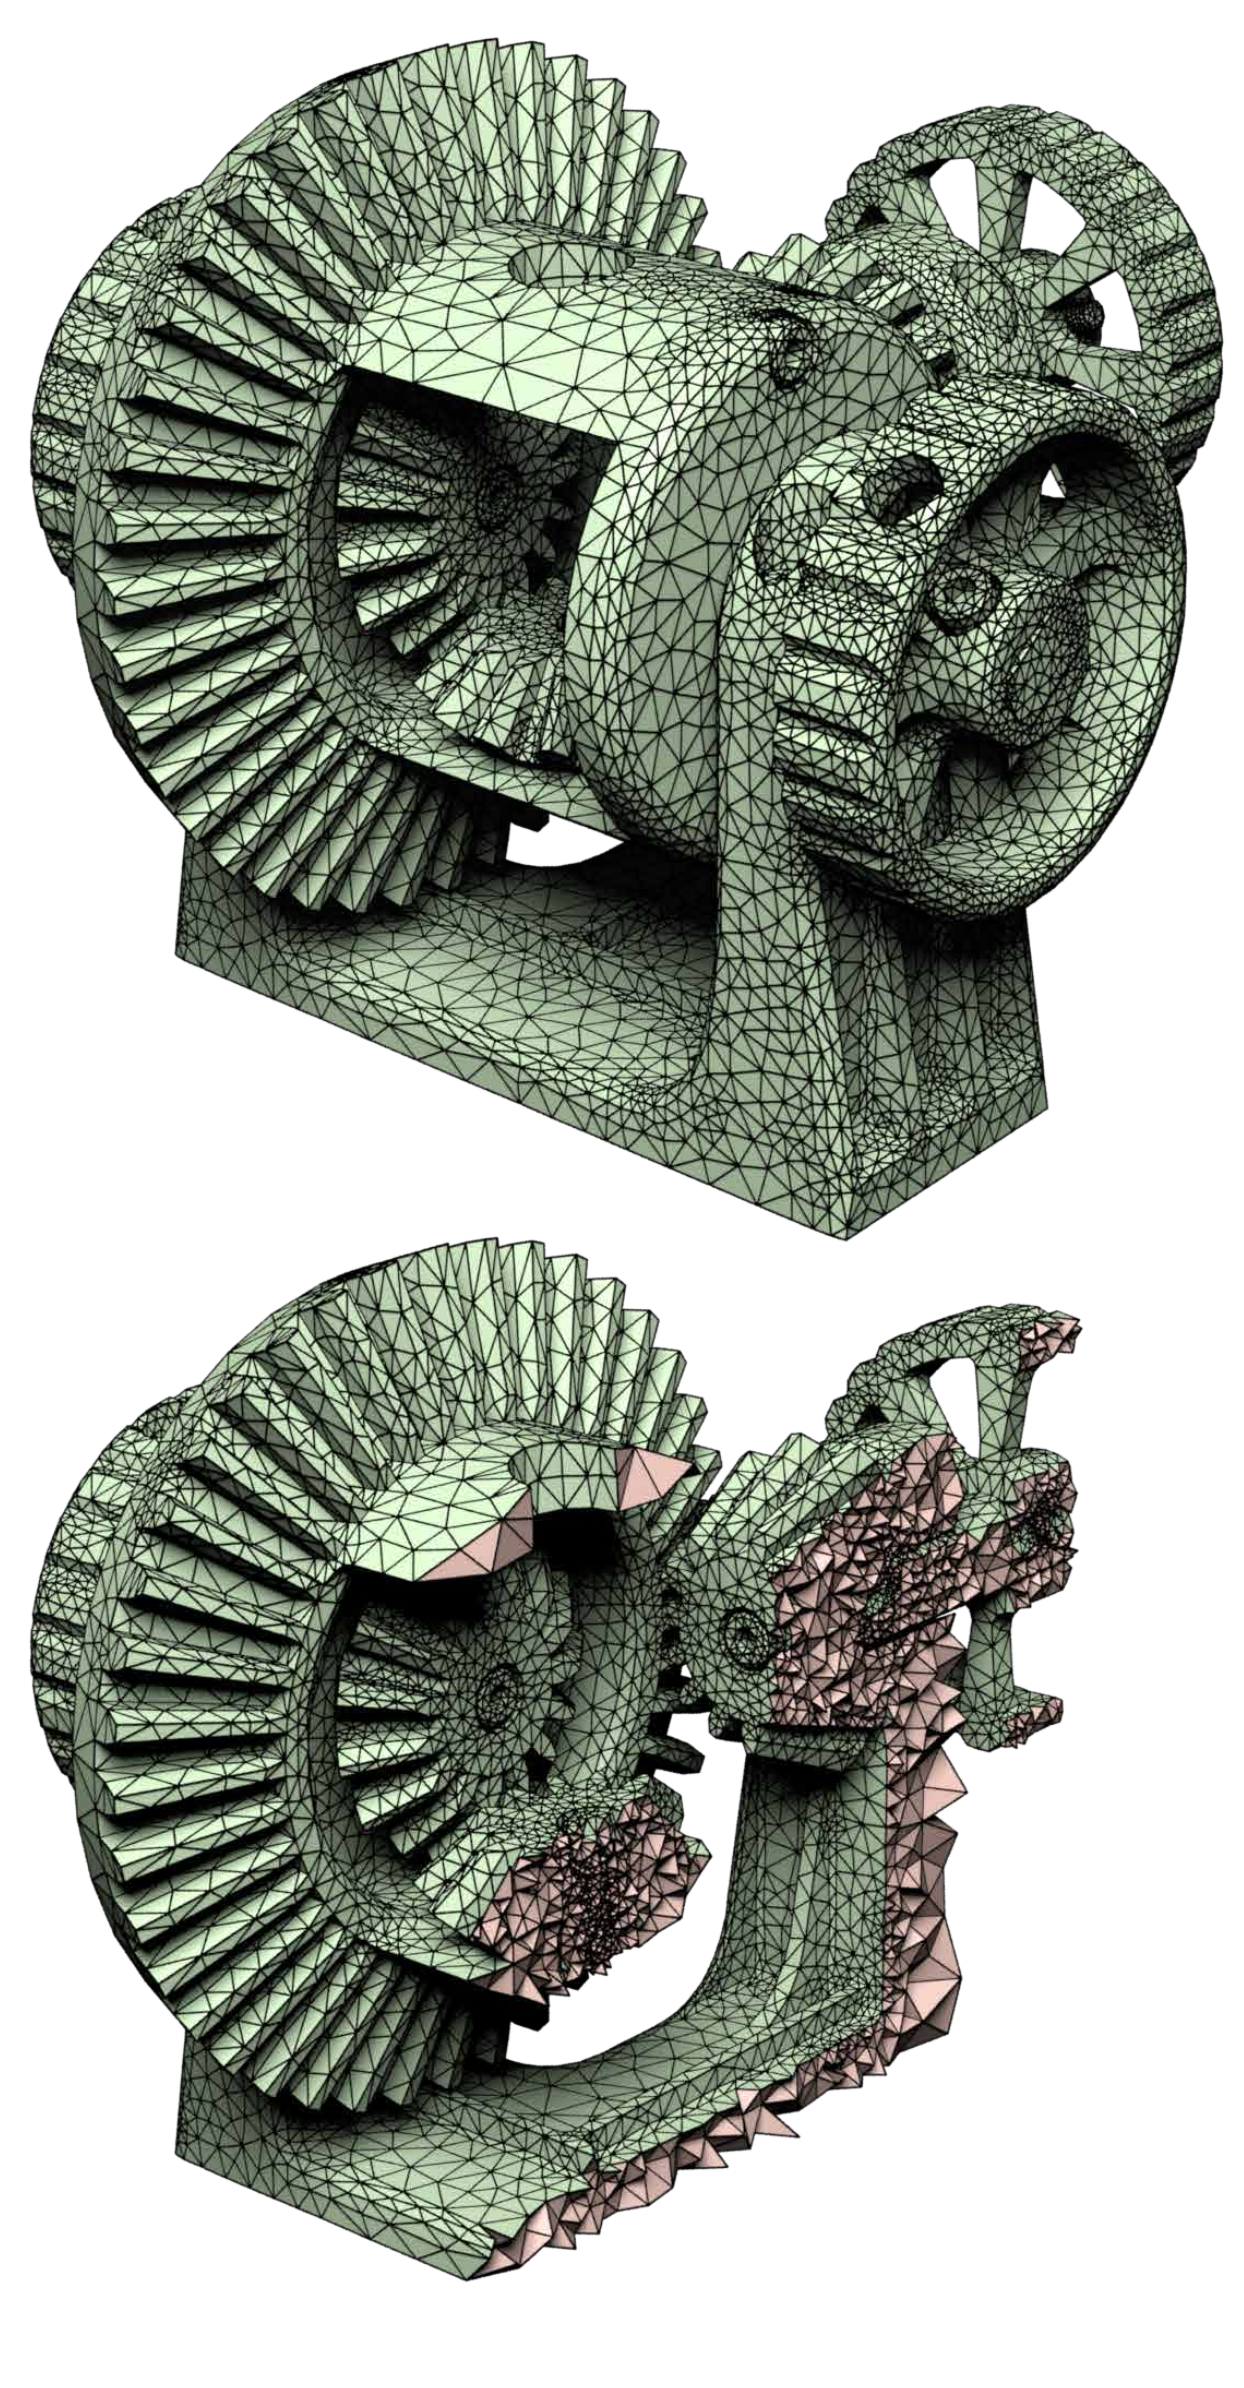
\includegraphics[width=2.5cm]{mesh_example_01.png}\\

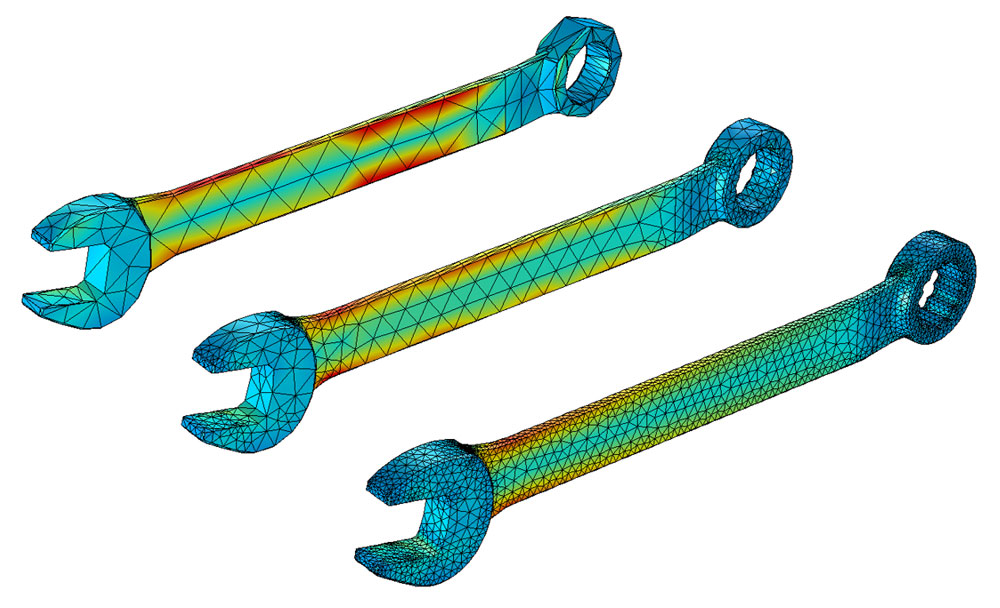
\includegraphics[width=4.0cm]{mesh_example_02.png}\\
\end{center}
\end{columns}
\blfootnote{Images from \cite{Hu2020}, \href{https://www.comsol.com/multiphysics/mesh-refinement}{Comsol}}
\end{frame}
\placelogotrue

\begin{frame}{Formulations}
\column{0.58\linewidth}
\centering
\begin{outline}
  \1 Begin with Strong Form 
  \1 
  \2 A finite collection of Elements
  \2 Track vertex connectivity
  \1 Elements can interpolate vertex values 
  \1 Meshing is a bottleneck
  \2 Expensive
  \2 Affects solution quality
\end{outline}

\column{0.38\linewidth}
\begin{center}
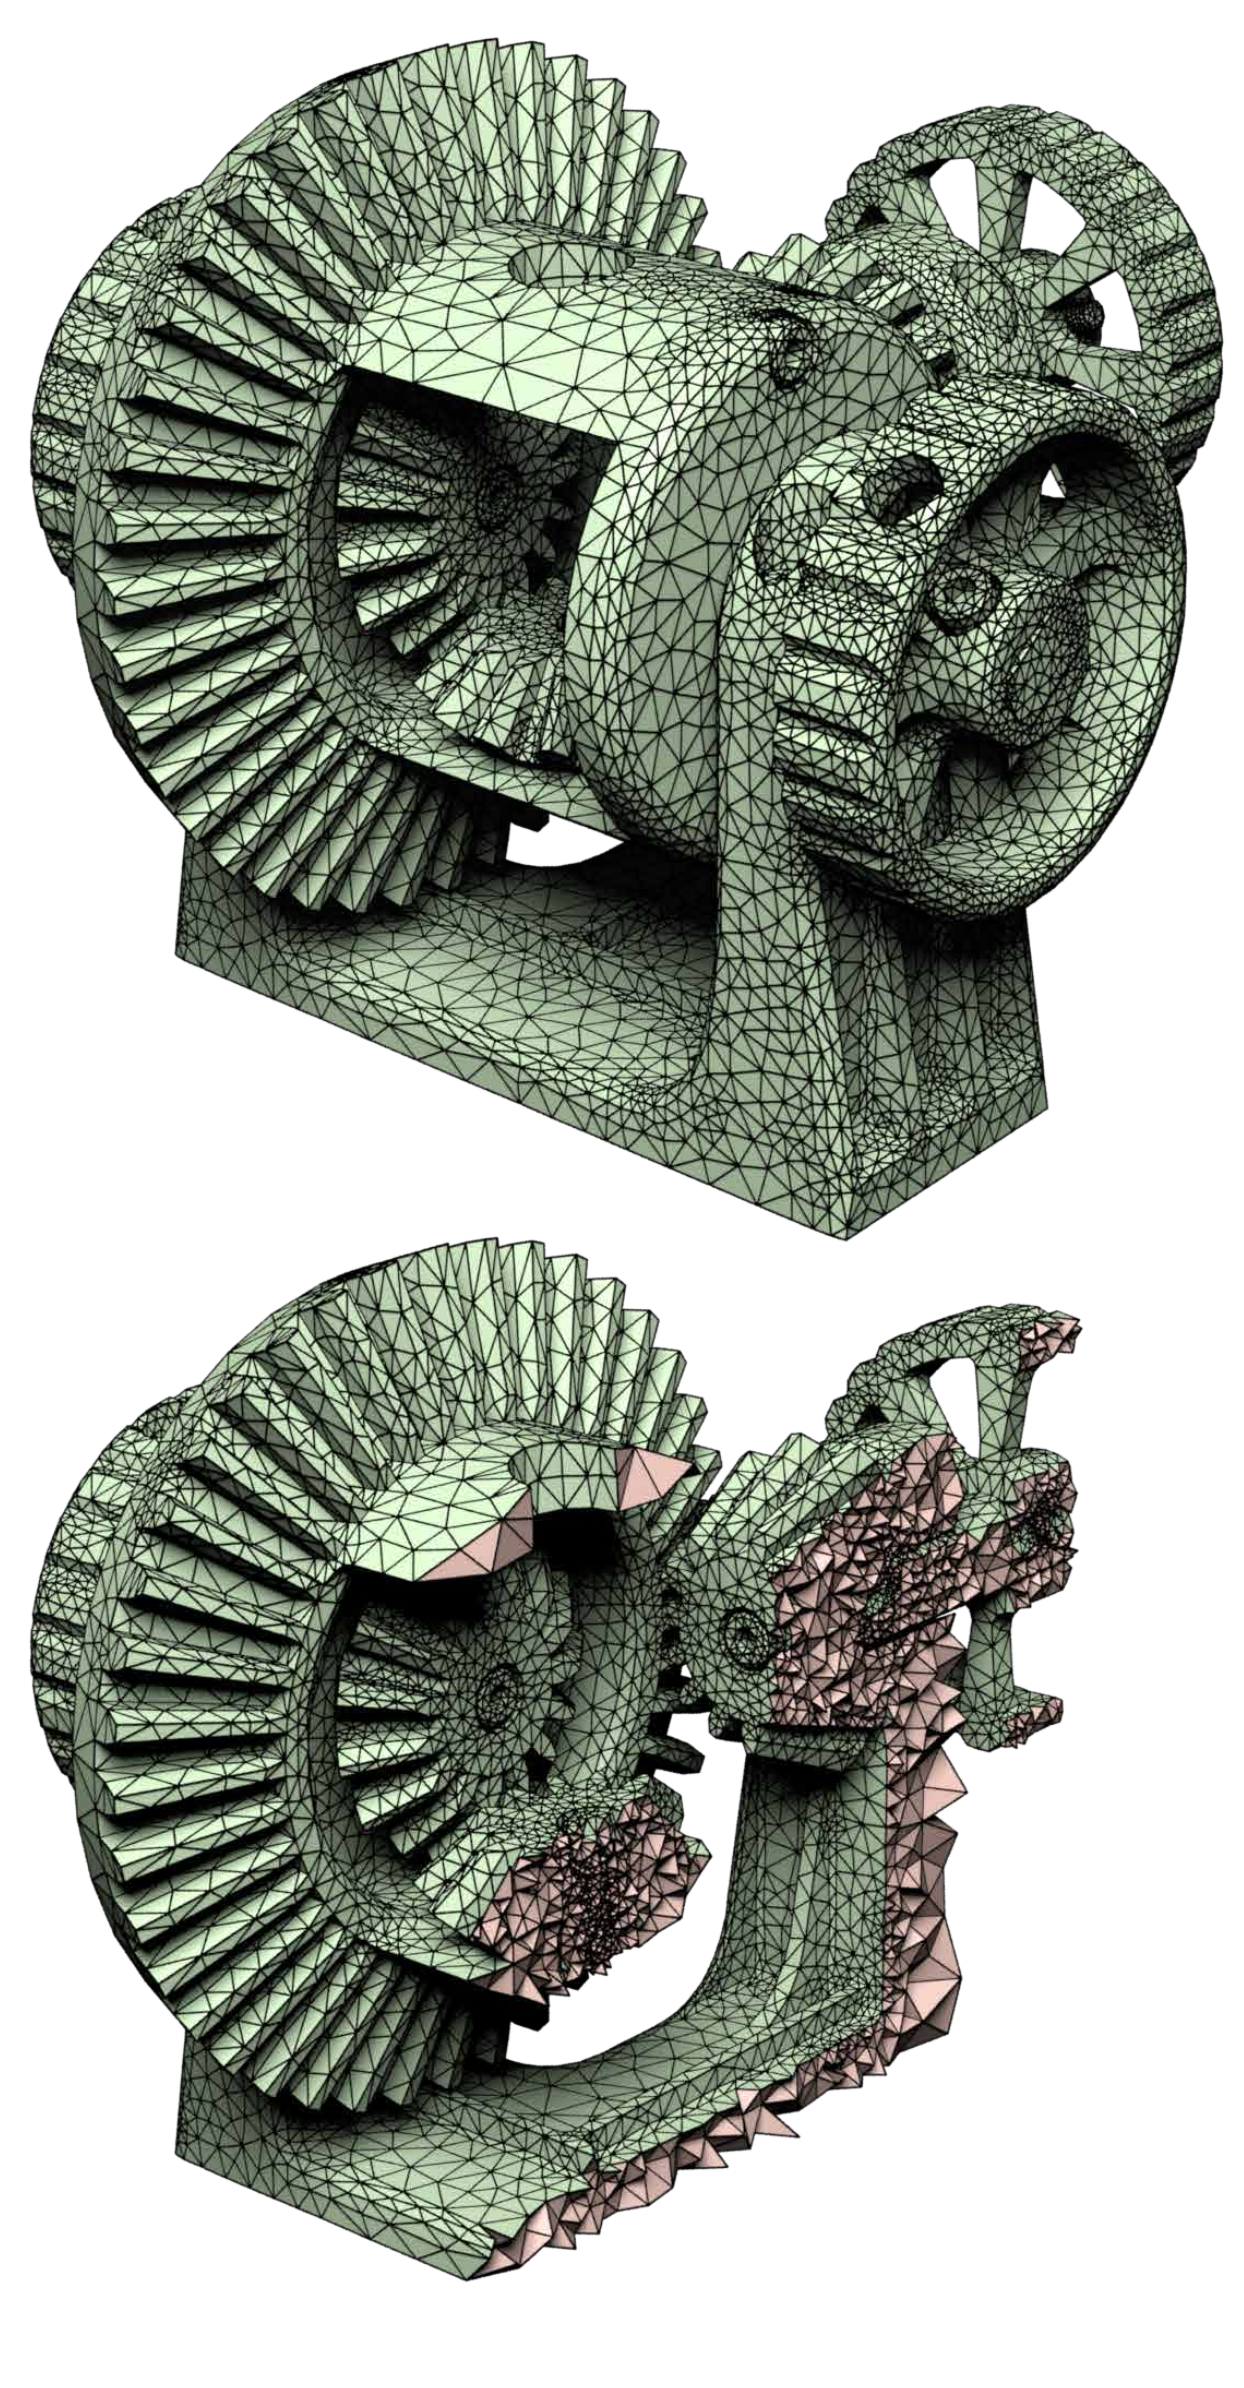
\includegraphics[width=2.5cm]{mesh_example_01.png}\\

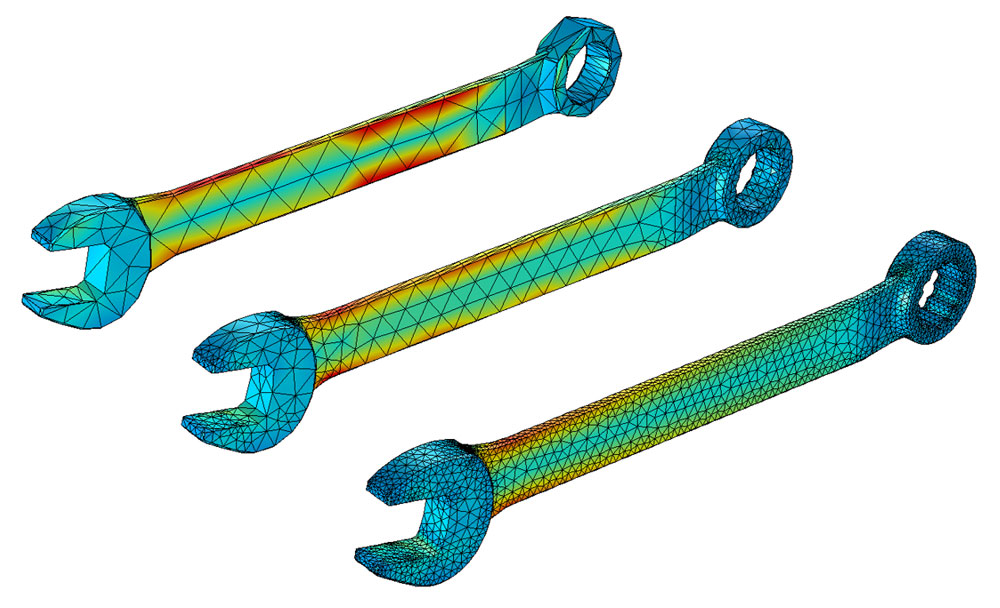
\includegraphics[width=4.0cm]{mesh_example_02.png}\\
\end{center}
\end{columns}
\end{frame}

% System Assembly

% Sparse Solve and solution
